%% Font size %%
\documentclass[11pt]{article}

%% Load the custom package
\usepackage{Mathdoc}

%% Numéro de séquence %% Titre de la séquence %%
\renewcommand{\centerhead}{Chap. 5 : Suites - Somme des termes d'une
  suite arithmétique}

%% Spacing commands %%
\renewcommand{\baselinestretch}{1} \setlength{\parindent}{0pt}

\begin{document}

\begin{exercice}[1][Sommes classiques]
\begin{multicols}{2}
\begin{enumerate}
\item Soit $w$ la suite arithmétique de premier terme $w_0 = 7$ et de
raison $10$.\\
Calculer
$\displaystyle S = w_0 + w_1 + ... + w_{20} =\sum_{k=0}^{k=20}w_k$.
\item Soit $w$ la suite arithmétique de premier terme $w_0 = 8$ et de
raison $4,5$.\\
Calculer
$\displaystyle S = w_{15} + w_{16} + ... + w_{40}
=\sum_{k=15}^{k=40}w_k$.
\columnbreak
\item Soit $v$ la suite arithmétique telle que $v_{60} = 3$ et de
raison $0,76$.\\
Calculer
$\displaystyle S = v_{4} + v_{5} + ... + v_{41} =\sum_{k=4}^{k=41}v_k$.
\item Soit $u$ la suite arithmétique telle que $u_8 = \dfrac{3}{2}$
et $u_{63} = \dfrac{45}{60}$.\\
Calculer
$\displaystyle S = u_{19} + u_{20} + ... + u_{42}
=\sum_{k=19}^{k=42}u_k$.
\end{enumerate}
\end{multicols}
\end{exercice}

\begin{exercice}[2][Avec critères de divisibilités]
\begin{enumerate}
\item Calculer la somme de tous les entiers naturels multiples de 3 inférieurs à 1 000.
\item Calculer la somme de tous les entiers naturels multiples de 5
inférieurs à 9 999.
\item Calculer la somme de tous les nombres entiers naturels
inférieurs à 2 154 ayant 3 comme chiffre des unités.
\end{enumerate}
\end{exercice}

\begin{exercice}[3][Problème de tuyaux]
\begin{multicols}{2}
Des tuyaux sont rangés comme indiqué ci-contre:
\begin{enumerate}
\item Quel est le nombre total de tuyaux dans un empilage de 5 couches ? 12 couches ?
\item On a stocké 153 tuyaux, combien y a-t-il de couches ?
\item Pour ranger 200 tuyaux, combien faut-il de couches ? Combien
reste t-il de tuyaux ?
\end{enumerate}
\columnbreak
\begin{center}
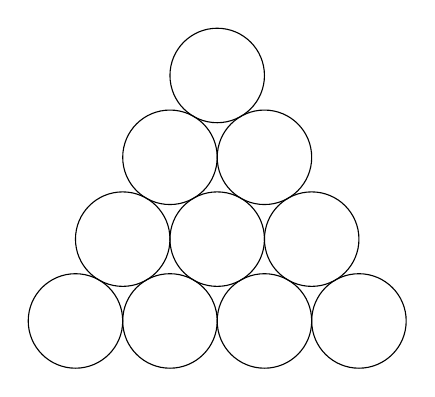
\begin{tikzpicture}
    % Define the radius of the circles
    \def\radius{0.6}

    % Define the vertical distance between rows
    \def\yshift{1.732*\radius}

    % Draw the first row
    \draw (0, 0) circle(\radius);

    % Draw the second row
    \draw (-\radius, -\yshift) circle(\radius);
    \draw (\radius, -\yshift) circle(\radius);

    % Draw the third row
    \draw (-2*\radius, -2*\yshift) circle(\radius);
    \draw (0, -2*\yshift) circle(\radius);
    \draw (2*\radius, -2*\yshift) circle(\radius);

    % Draw the fourth row
    \draw (-3*\radius, -3*\yshift) circle(\radius);
    \draw (-\radius, -3*\yshift) circle(\radius);
    \draw (\radius, -3*\yshift) circle(\radius);
    \draw (3*\radius, -3*\yshift) circle(\radius);
\end{tikzpicture}
\end{center}
\end{multicols}
\end{exercice}

\begin{exercice}[4][Manipulation de la formule]
Soit \((u_n)\) une suite arithmétique de raison \(r\), de premier terme \(u_1\) et de \(n\)-ième terme \(u_n\). \\
On note \(S_n = u_1 + u_2 + \cdots + u_n\). \\
Les questions sont indépendantes les unes des autres.
\begin{enumerate}
\item Calculer \(u_1\) et \(S_{17}\) lorsque : $u_{17} = 105 \quad \text{et} \quad r = 2$
\item Calculer \(u_1\) et \(u_{33}\) lorsque : $r = -7 \quad \text{et} \quad S_{33} = 0$
\item Calculer \(n\) et \(u_1\) lorsque : $u_n = 14, \quad r = 7 \quad \text{et} \quad S_n = -1176$
\end{enumerate}
\end{exercice}



\end{document}
